\section{Turning on \& Blinking a LED}\label{sec:Turning on a LED} % (fold)
\subsection{Source Code}
\begin{code}
    \caption{Turning on a LED using Arduino Framework}
    \begin{minted}[frame=single, linenos]{cpp}
#include <Arduino.h>

#define LED_PIN PA15

void setup() {
  pinMode(LED_PIN, OUTPUT);
}

void loop() {
  digitalWrite(LED_PIN,HIGH);
}
\end{minted}
    \label{code:ledon}
\end{code}
\begin{minted}{cpp}

\end{minted}
\begin{code}
    \caption{Blinking a LED with a interval of one second}
    \begin{minted}[frame=single, linenos]{cpp}
#include <Arduino.h>

#define LED_PIN PA15

void setup() {
  pinMode(LED_PIN, OUTPUT);
}

void loop() {
  digitalWrite(LED_PIN,HIGH);
  delay(1000);
  digitalWrite(LED_PIN,LOW);
  delay(1000);
}
\end{minted}
    \label{code:blink}
\end{code}
\begin{minted}{cpp}

\end{minted}
% section Turning on a LED (end)

\subsection{Circuit Diagram}
\begin{figure}[h]
    \centering
\begin{circuitikz}
    \draw 
        (0,0) node[vcc]{+5V/A15} % Power source
        to[R, l=220 $\Omega$] (4,0)
        to[led] (5,0)
        to[short] (6,0)
        to node[sground]{GND} (6,-1);
\end{circuitikz}
\caption{Simple LED circuit diagarm}
\label{fig:cir}
\end{figure}
\newpage
\subsection{Simulation in TinkerCAD}
\begin{figure}[ht]
    \centering
    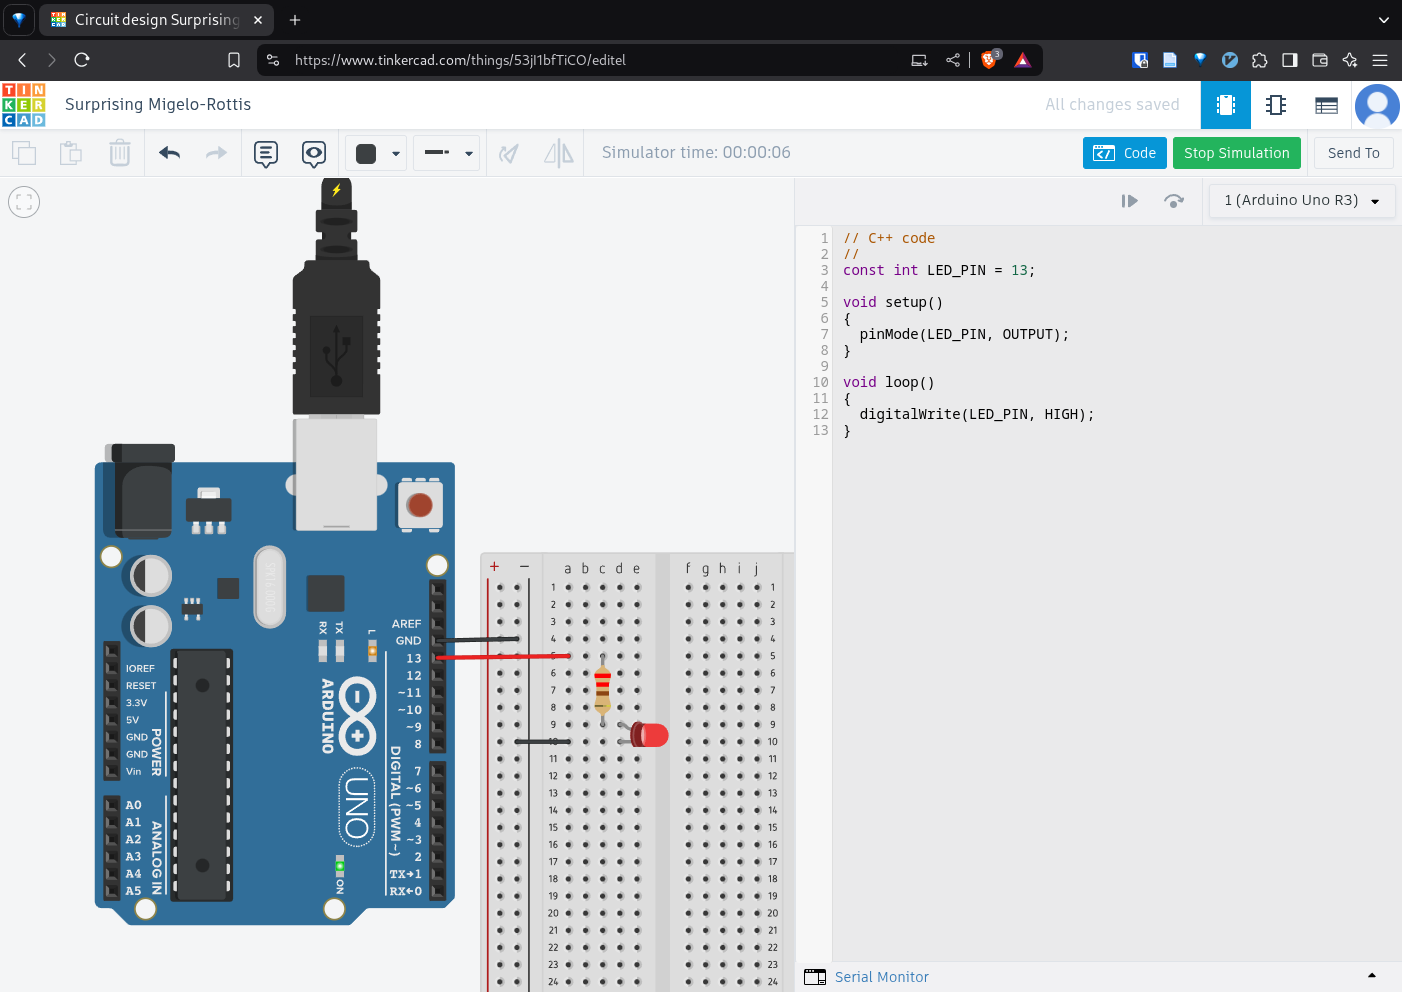
\includegraphics[width=0.95\textwidth]{img/tinkercad.png}
    \caption{Simulating the circuit using Arduino in TinkerCAD}\label{fig:sim}
\end{figure}
\section{Discussion}
I successfully implemented the circuit in \cref{fig:cir} using 
the STM32F103C8T6 microcontroller board. The STM32 has multiple GPIO pins that
can be used as digital output pin. Among these pins, I chose the A15 pin which was referenced as \texttt{PA15} in \cref{code:ledon} and \cref{code:blink}.

The code was implemented using the Arduino framework which gives various 
built-in functions to interact with the microcontroller. Using \texttt{pinMode}
function the PA15 pin was set as an ouptut pin inside the \texttt{setup} function. 
To turn on the LED the pin was set to HIGH using the function \texttt{digitalWrite}.
In case of blinking, the pin was continuously set to HIGH and LOW with a
delay of 1000ms or 1s using the \texttt{delay} function.

Finally, the code was uploaded to the microcontroller using stlink protocol.
To simulate the same actions virtually, tinkerCAD platform was used. There I 
used the Arduino UNO R3 as the microcontroller board. And the digital pin 13 
was used for the LED pin. Using the similar code, I ran the simulation, see \cref{fig:sim}
